\documentclass[11pt,a4paper]{article}
\usepackage[margin=2.3cm]{geometry}
\usepackage{graphicx,booktabs,amsmath,xcolor,tabularx,enumitem,listings}
\usepackage[version=4]{mhchem}
\usepackage[most]{tcolorbox}
\usepackage[hidelinks]{hyperref}
\graphicspath{{figures/}}
\setlist{itemsep=2pt,topsep=3pt}
\setlength{\parskip}{4pt}

% --- status markers: change \torun to \done once a lab has been run yourself
\newcommand{\done}{\textcolor{green!45!black}{\textbf{Completed}}}
\newcommand{\torun}{\textcolor{orange!80!black}{\textbf{Reference values --- to rerun}}}

\newtcolorbox{matters}{colback=blue!4,colframe=blue!50!black,boxrule=0.6pt,arc=2pt,
  left=6pt,right=6pt,top=3pt,bottom=3pt,fonttitle=\bfseries\small,title=Why this matters for the project}
\lstset{basicstyle=\ttfamily\small,columns=fullflexible,keepspaces=true,breaklines=true,
  aboveskip=2pt,belowskip=2pt}

\newcommand{\lab}[3]{\section{#1}\noindent\textbf{Status:} #2 \qquad \textbf{Molecule(s):} #3\par}

\title{DFT study report: test calculations before the photocatalyst project}
\author{Lindejiade}
\date{October 2026}

\begin{document}
\maketitle

\noindent\textbf{Purpose.} The photocatalyst project computes the electronic structure of 16
organic photocatalysts with DFT. Before working with its pipeline, I ran a series of small test
calculations. Each one is on a molecule whose answer is known, so I could understand what each
step does and check that the method behaves as expected. Every calculation uses the project's
level of theory: \textbf{B3LYP/def2-SVP in PySCF}, with ddCOSMO water where stated. Lessons~3--5
are in the exercise notebook \texttt{dft\_exercises\_L3-5.ipynb}, where each result is checked
against a reference value.

\begin{center}\small
\begin{tabularx}{\linewidth}{@{}clXl@{}}
\toprule
& Test & Question & Status \\
\midrule
1 & First DFT calculation & What do the basis set and functional control? & \torun \\
2 & Geometry optimisation & What do ``optimised'' and ``converged'' mean? & \torun \\
3 & Orbitals, IE and TDDFT & What do HOMO/LUMO energies mean, and not mean? & \done \\
4 & SMILES $\to$ DFT & How does a string become a computable molecule? & \done \\
5 & Charge and solvent & Why compute eosin~Y as $-2$, and in water? & \torun \\
6 & Reproduce the project & Can I reproduce a project result myself? & \torun \\
\bottomrule
\end{tabularx}
\end{center}

%=============================================================================
\lab{Test 1 --- First DFT calculation}{\torun}{water}

\textbf{What I ran.} Single points at the experimental geometry with three basis sets (STO-3G,
def2-SVP, def2-TZVP) and three methods (HF, PBE, B3LYP).

\textbf{Result.} Total energy fell by 1.1~Ha (about 3000~kJ/mol) from STO-3G to def2-TZVP, and
changed by about 0.4~Ha between HF and B3LYP. The HOMO energy was $-13.8$~eV with HF but
$-8.6$~eV with B3LYP (def2-TZVP). The experimental ionisation energy is 12.6~eV.

\textbf{What I learned.} A total energy has no meaning on its own. Only energy differences at the
\emph{same} level of theory are meaningful. Orbital energies depend strongly on the functional.

\begin{matters}
Every number in the project must be labelled with its level of theory and compared only with
numbers computed the same way. This is why all 16 molecules use one functional, one basis set and
one solvent.
\end{matters}

%=============================================================================
\lab{Test 2 --- Geometry optimisation}{\torun}{water, benzene}

\textbf{What I ran.} DFT optimisations starting from force-field structures.

\textbf{Result.} Water: O--H 0.967~\AA, H--O--H 103.1$^\circ$ (experiment 0.958~\AA,
104.5$^\circ$). Benzene: C--C 1.398~\AA\ (experiment 1.397~\AA), converged in 4 cycles from the
MMFF start.

\textbf{What I learned.} An optimisation alternates between an SCF (energy and forces) and a step
downhill. ``Converged'' means both the forces and the step size are below thresholds. A good
starting geometry saves expensive DFT steps.

\begin{matters}
The project starts every molecule from a force-field (MMFF) geometry. For rigid molecules this is
already close to DFT. For the flexible and charged dyes (eosin~Y, rhodamine~B, riboflavin) it was
0.17--0.40~\AA\ off, and eosin~Y's very flat twist needed relaxed convergence criteria.
\end{matters}

%=============================================================================
\lab{Test 3 --- Orbitals, ionisation energy and TDDFT}{\done}{benzene}

\textbf{What I ran.} (a)~A B3LYP single point and its orbital energies. (b)~The ionisation energy
three ways. (c)~Orbital pictures with \texttt{cubegen}. (d)~TDDFT for the lowest three excited
states.

\textbf{Results.}
\begin{center}\small
\begin{tabular}{@{}lr@{\qquad}lr@{}}
\toprule
\multicolumn{2}{@{}l}{Ionisation energy (eV)} & \multicolumn{2}{l}{Excitations (eV)} \\
\midrule
Experiment & 9.24 & HOMO--LUMO gap & 6.72 \\
$-$HOMO, B3LYP & 6.97 & TDDFT S$_1$ ($f = 0.000$) & 5.48 \\
$-$HOMO, HF & 9.17 & TDDFT S$_3$ ($f = 0.589$) & 7.28 \\
$\Delta$SCF, B3LYP & \textbf{9.24} & Experiment: weak / strong band & 4.9 / $\sim$6.9 \\
\bottomrule
\end{tabular}
\end{center}
HOMO/HOMO$-1$ ($-6.97$~eV) and LUMO/LUMO$+1$ ($-0.25$~eV) are degenerate pairs.

\begin{figure}[h]
\centering
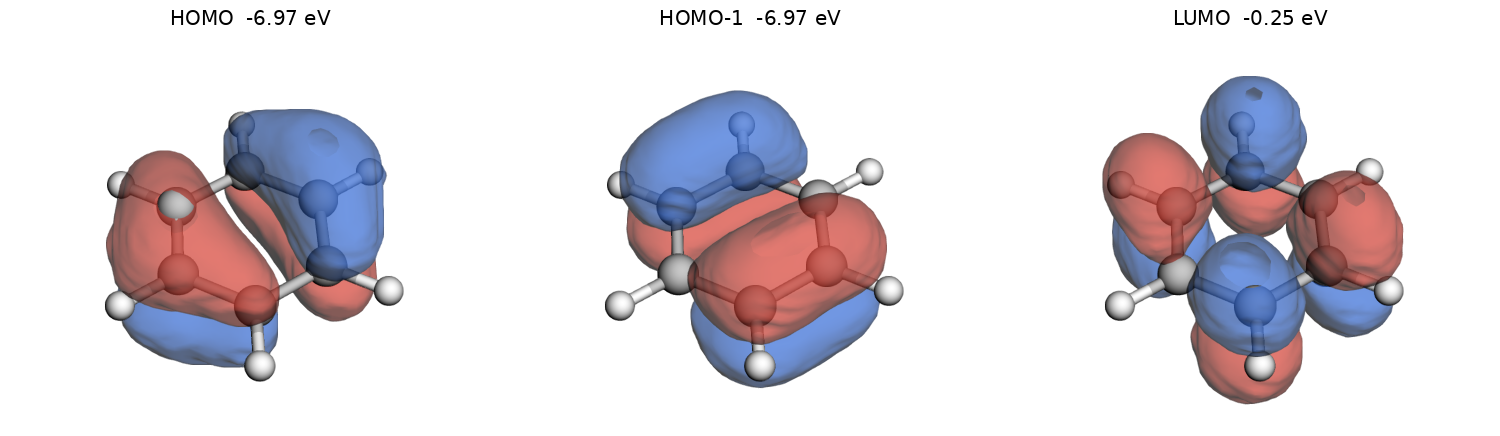
\includegraphics[width=0.7\linewidth]{benzene_frontier.png}
\caption{Benzene HOMO, HOMO$-1$, LUMO ($\pm$0.03~a.u.).}
\end{figure}

\textbf{What I learned.}
\begin{itemize}
  \item \textbf{Self-interaction error.} B3LYP's $-$HOMO underestimates the ionisation energy by
  2.3~eV, because each electron partly repels itself. This pushes occupied orbital energies up.
  $\Delta$SCF, which subtracts the total energies of the cation and the neutral molecule, cancels
  most of this error and matches experiment.
  \item \textbf{Three different gaps.} The KS gap (6.72~eV) is an orbital difference. The
  fundamental gap (ionisation energy minus electron affinity, $\approx$10.4~eV) needs the ions.
  The optical gap (4.9~eV) is the lowest absorption, and it is smallest because the excited
  electron and the hole still attract each other.
  \item \textbf{TDDFT} computes real excitations. Each comes with an oscillator strength $f$:
  $f = 0$ means a dark (symmetry-forbidden) state. That is why benzene's lowest band is so weak.
  S$_1$ is three times closer to experiment than the KS gap.
  \item \texttt{cubegen} only converts orbital coefficients into a 3D grid for viewing. It changes
  no results.
  \item Members of a degenerate pair must not be interpreted alone.
\end{itemize}

\begin{matters}
The project's energy-level diagram uses B3LYP HOMO/LUMO energies, so it can show trends between
dyes but not real ionisation energies or redox potentials. That is why the water-splitting
reference lines were removed from it. The project's comparison with experiment ($r = 0.90$, MAE
0.45~eV) uses the KS gap as a stand-in for absorption; \textbf{the project does not use TDDFT
yet}, and this test shows it is needed. In Mes-Acr$^+$ the three highest occupied orbitals lie
within 13~meV of each other, so the warning about degenerate orbitals applies there too.
\end{matters}

%=============================================================================
\lab{Test 4 --- From SMILES to a DFT calculation}{\done}{benzene, anthraquinone}

\textbf{What I ran.} I wrote my own \texttt{smiles\_to\_atoms} function (SMILES $\to$ add H $\to$
ETKDG 3D embedding $\to$ MMFF $\to$ list of atoms and coordinates), then ran DFT single points in
vacuum and in water.

\begin{lstlisting}
m = Chem.MolFromSmiles(smiles); q = Chem.GetFormalCharge(m)
mh = Chem.AddHs(m); AllChem.EmbedMolecule(mh, params); AllChem.MMFFOptimizeMolecule(mh)
atoms = [(a.GetSymbol(), tuple(pos[i])) for i, a in enumerate(mh.GetAtoms())]
mol = gto.M(atom=atoms, basis="def2-svp", charge=q, spin=0)
\end{lstlisting}

\textbf{Results.} Benzene's MMFF geometry gave C--C 1.395~\AA, and a HOMO only 0.008~eV different
from the DFT-optimised geometry. Anthraquinone:

\begin{center}\small
\begin{tabular}{@{}llrrr@{}}
\toprule
Geometry & Solvent & HOMO (eV) & LUMO (eV) & Gap (eV) \\
\midrule
MMFF (mine) & vacuum & $-7.170$ & $-2.976$ & 4.194 \\
MMFF (mine) & water & $-7.288$ & $-3.022$ & 4.266 \\
DFT-optimised (project) & water & $-7.314$ & $-3.041$ & 4.273 \\
\bottomrule
\end{tabular}
\end{center}

\textbf{What I learned.}
\begin{itemize}
  \item \texttt{MolFromSmiles} returns a \emph{graph} (atoms, bonds, charges) with no coordinates
  and only implicit hydrogens. A broken SMILES returns \texttt{None} without an error.
  \item DFT receives only nuclei, coordinates, charge and spin, plus the method choices. It never
  sees bonds or SMILES.
  \item For rigid anthraquinone the geometry difference (MMFF vs DFT) shifts the gap by only
  0.007~eV, and the solvent shifts the orbitals by only about 0.1~eV, because the molecule is
  neutral with almost no dipole.
\end{itemize}

\begin{matters}
This is exactly what the project's Step~1 does (plus conformer search and checks), so I can now
read that script. It also explains why MMFF geometries are acceptable for rigid neutral dyes but
not automatically for the flexible or charged ones.
\end{matters}

%=============================================================================
\lab{Test 5 --- Charge and solvent}{\torun}{phenol, phenolate}

\textbf{What I ran.} Phenol and phenolate (\ce{C6H5O-}) in vacuum and in ddCOSMO water. I also
built phenolate once with the charge deliberately left out.

\textbf{Results.}
\begin{center}\small
\begin{tabular}{@{}lrrr@{}}
\toprule
& HOMO vacuum (eV) & HOMO water (eV) & Solvent shift (eV) \\
\midrule
phenol (neutral) & $-6.18$ & $-6.26$ & $-0.08$ \\
phenolate ($-1$) & $+0.32$ & $-4.15$ & $-4.47$ \\
\bottomrule
\end{tabular}
\end{center}
Without the charge, PySCF refused: 49 electrons cannot all be paired.

\textbf{What I learned.} In vacuum the anion's extra electron is not bound (positive HOMO). Water
stabilises the ion by 4.5~eV but the neutral molecule by only 0.08~eV, because the solvent
responds to charge. For a \emph{dianion}, losing the charge removes two electrons, the count stays
even, and no error appears.

\begin{matters}
Eosin~Y, rose bengal and fluorescein are dianions. They must be computed with charge $-2$ and in
solvent, or their orbitals are meaningless. The same silent failure happens with the project's own
file: reading \texttt{eosinY.xyz} directly into PySCF gives charge 0 and 306 electrons instead of
308, with no warning. That is why the project stores the charge in every xyz file and passes it
explicitly. Using water for \emph{every} molecule also keeps all 16 computed at the same level of
theory, so they can be compared fairly.
\end{matters}

%=============================================================================
\lab{Test 6 --- Reproducing a project result}{\torun}{anthraquinone}

\textbf{What I ran.} A single point with my own code on the project's DFT-optimised anthraquinone
geometry, in water.

\textbf{Result.} HOMO $-7.3138$, LUMO $-3.0409$~eV: identical to the project's
\texttt{frontier\_orbitals.csv} to four decimal places.

\begin{matters}
The project's Step~3 is this calculation in a loop over 16 molecules. Reproducing one row
independently is the basic check that the pipeline does what I think it does.
\end{matters}

%=============================================================================
\section{Mistakes I made and what they taught me}
\begin{itemize}
  \item \textbf{Units.} My first $\Delta$SCF ionisation energy for benzene was 0.34. The value was
  correct but in Hartree: $0.34 \times 27.211 = 9.24$~eV. PySCF always returns Hartree.
  \item \textbf{Wrong molecule.} I used naphthalene's SMILES for anthraquinone. Everything ran;
  the giveaway was 68 electrons instead of 108. A wrong SMILES is still a valid SMILES, so
  results must be checked against an independent fact such as the molecular formula. The project
  does this for every molecule.
\end{itemize}

\section{Summary and next steps}

\textbf{Main things I learned.} Compare only energy differences at the same level of theory.
B3LYP orbital energies give trends, not absolute ionisation energies or redox potentials.
Absorption needs TDDFT. The charge must be passed explicitly, because losing two charges fails
silently. Ions need a solvent model. And every result should be checked against something
independent.

\textbf{Next steps.}
\begin{enumerate}
  \item Rerun Tests 1, 2, 5 and 6 myself.
  \item Run TDDFT on anthraquinone and compare with its measured 325~nm band (the first step
  towards adding TDDFT to the project).
  \item Rerun the project's Step~3 on the three newly optimised dyes, then Step~5, to see whether
  the geometry changes their orbital energies.
\end{enumerate}

\textbf{Questions for my PI.}
\begin{itemize}
  \item Which functional does the group use for TDDFT on dyes, especially charge-transfer ones?
  \item Should each molecule be computed in its experimental solvent rather than water?
  \item How does the group usually compute redox potentials ($\Delta$SCF in solvent, or another
  approach)?
\end{itemize}

\end{document}
